\subsection{OB-11 (ASB)}
LAN z hlediska kybernetické bezpečnosti. Zranitelnosti protokolů rodiny TCP/IP. Zabezpečení sítí LAN na úrovni síťových zařízení (switche, routery, firewally). Využití technologie VLAN.

\subsubsection*{model CIA}
\begin{itemize}
	\item Confidentiality (Důvěrnost)
	\begin{itemize}
		\item porušení důvěrnosti: odposlech síťového provozu
		\item různá úroveň informací v závislosti na vrstvě: aplikační (čtení uživatelských dat), transportní (informace o protistranách a službě), síťová (protistrany, typ transportního protokolu, velikost), ...
		\item nemusí jít vždy jen o uživatelská data, ale např informace směrovacích protokolů
	\end{itemize}
	\item Integrity (Integrita)
	\begin{itemize}
		\item data jsou nezměněna v průběhu přenosu
		\item porušení integrity: úprava přenášených dat
	\end{itemize}
	\item Availability (Dostupnost)
	\begin{itemize}
		\item běžící služba, přenos dat sítí (prostě to funguje)
		\item porušení dostupnosti: DoS (Denial of Service)
	\end{itemize}
\end{itemize}

\subsubsection*{Bezpečnost síťových protokolů}
\begin{itemize}
	\item Ethernet
	
	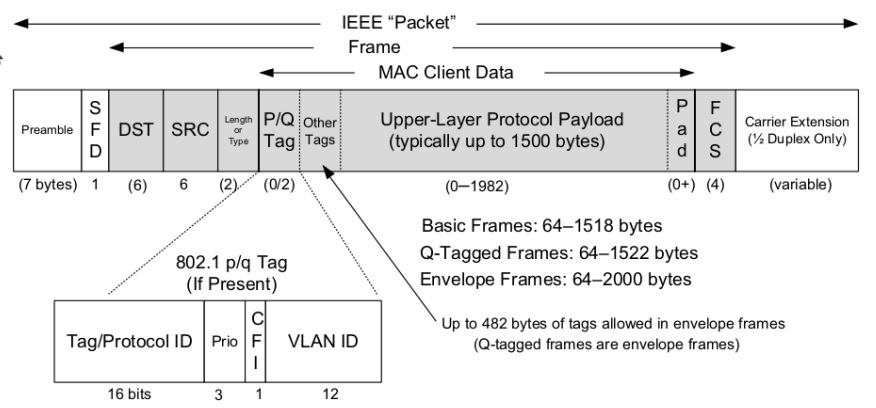
\includegraphics[width=0.8\textwidth]{img/OB-11_0.jpg}
	
	\begin{itemize}
		\item otevřená (plaintext) komunikace
		\item zajišťuje doručení dat (kontrolní součty), ale data lze jak odposlouchávat tak měnit
		\item u protokolu CSMA/CD lze udělat DoS (místo náhodné doby čekání prostě vysílat hned)
		\item lze použít VLAN --- k packetům se přidají tagy (do jaké VLAN packet patří) --- max 4094 VLAN (12 bitů, 2 rezervované hodnoty) --- rozdělení broadcastové domény
	\end{itemize}
	
	\item IP
	
	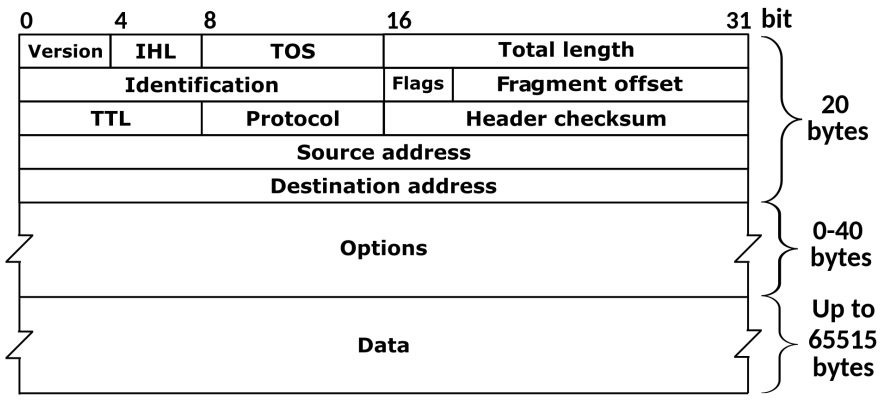
\includegraphics[width=0.7\textwidth]{img/OB-11_1.jpg}
	
	\begin{itemize}
		\item otevřená (plaintext) komunikace
		\item pouze zapouzdření a přenos dat, neřeší ani správné doručení
		\item kontrola integrity musí být zajištěna vyšší vrstvou
		\item IP adresu lze podvrhnout
	\end{itemize}
	
	\item UDP
	\begin{itemize}
		\item v hlavičce prakticky jen zdroj, cíl a checksum
		\item slouží pouze k zapouzdření dat, není garantováno pořadí
		\item integritu musí řešit vyšší vrstva
		\item nenáročný na správu spojení (lze využít k DDoS)
	\end{itemize}
	
	\item TCP
	
	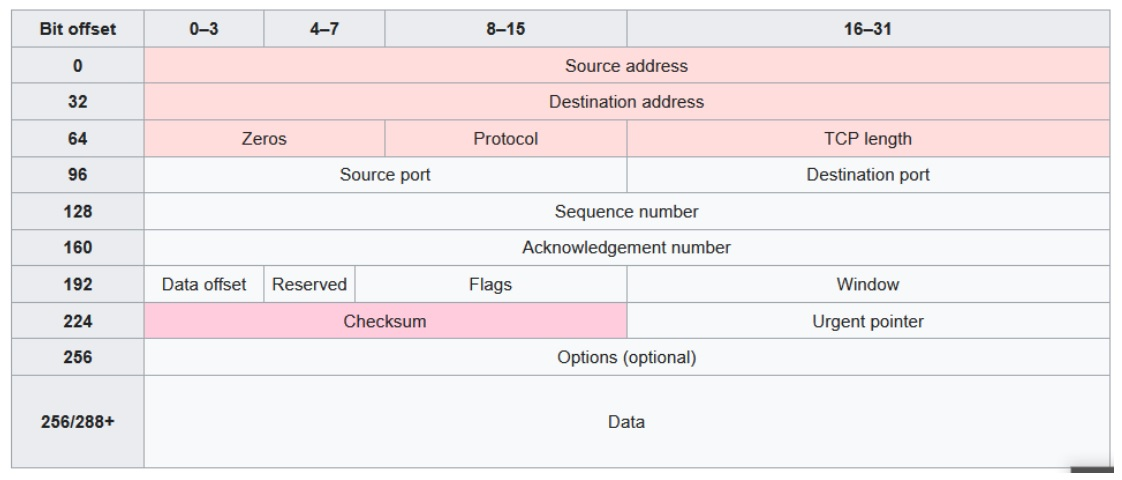
\includegraphics[width=0.7\textwidth]{img/OB-11_2.jpg}
	
	\begin{itemize}
		\item slouží pro doručení v pořadí, neřeší integritu
		\item integritu musí řešit vyšší vrstva
		\item komunikující uzly si musí uchovávat informaci o stavu spojení --- lze využít k SYN Flood DoS útoku
	\end{itemize}
	
	\item ARP
	\begin{itemize}
		\item ARP cache --- každý uzel si zapisuje příchozí odpovědi (jakékoliv)
		\item ARP Spoofing --- podvržení linkové adresy
		\item ARP Cache Poisonong --- zneužití ARP Cache oběti pomocí spoofingu --- výsledkem je zasílání dat na špatnou linkovou adresu, umožňuje získat pozici MitM (Man in the Middle)
		\item obrana: static ARP, kontrola na portu switche
	\end{itemize}
	
	\item DHCP
	\begin{itemize}
		\item DHCP server přiděluje dynamicky konfiguraci sítě zařízením
		\item rogue DHCP server --- DHCP server navíc, může vzniknout špatnou konfigurací, nebo útokem
		\item obrana: DHCP Snooping na switch portu, filtrování DHCP komunikace
	\end{itemize}
	
	\item ICMP
	\begin{itemize}
		\item nepřenáší data vyšší vrstvy, ale může přímo i nepřímo sloužit k útokům
	\end{itemize}
\end{itemize}

\subsubsection*{Bezpečnost síťových zařízení}
\begin{itemize}
	\item hub
	\begin{itemize}
	\item pracuje na fyzické vrstvě, přeposílá vstup
		\item dnes už se moc nesetkáváme, překonané zařízení
		\item bezpečnost 0, rozšiřuje kolizní doménu, každá stanice "slyší" vše co se v dané kolizní doméně děje, může způsobovat kolize úmyslně
	\end{itemize}
	\item switch
	\begin{itemize}
		\item pracuje na linkové vrstvě
		\item rámce jsou přeposílány na konkrétní port na základě paměti switche
		\item broadcast přeposílán všude
		\item odděluje kolizní domény, nedochází ke kolizím
		\item možnosti útoků typu ARP spoofing  / MAC floding
		\item široké možnosti bezpečné konfigurace switche
		\begin{itemize}
			\item vypnutí nepoužitých portů / zásuvek (aby se do volné zásuvky nemohl připojit kdokoliv)
			\item limit počtu MAC adres na portu (obrana proti MAC flooding)
			\item VLAN --- logické členění síťových segmentů, rozdělení broadcastových domén (útok VLAN hopping --- switch spoofing, pc se tváří jako switch a chce nastavit trunk spojení / double tagging, přidání extra vlan tagu)
			\item spanning tree protocol --- potřeba nastavit, aby se nemohl připojit nový (útočníkův) switch
			\item lze nastavit ochranu proti DHCP spoofingu
		\end{itemize}
	\end{itemize}
	\item router
	\begin{itemize}
		\item možnost nastavení ACL
	\end{itemize}
	\item firewall
	\begin{itemize}
		\item možnost nastavení ACL
	\end{itemize}
	\item IDS (Intrusion detection system)
	\item IPS (Intrusion prevention system)
\end{itemize}